% Vektorgrafiken ausschließlich für die Lesefassung.
% Die erste Grafik ist eine Zielspezifikation, die zweite zeigt nur
% den lokalen Induktionsschritt; keine setzt den Rekursionssatz voraus.
\definecolor{dedekindblue}{RGB}{34,92,133}
\definecolor{dedekindred}{RGB}{163,49,45}
\definecolor{dedekindshade}{RGB}{226,237,244}

\newcommand{\DedekindRecursionDiagram}{%
  \par\medskip\noindent
  \begin{minipage}{\linewidth}
  \centering
  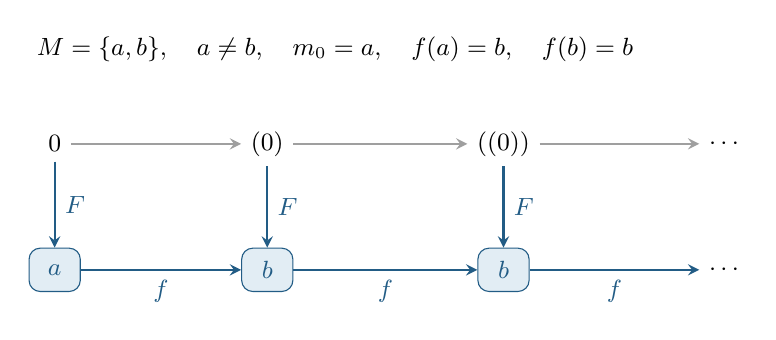
\begin{tikzpicture}[x=1cm,y=1cm,font=\small,>=stealth,
    value/.style={draw=dedekindblue,fill=dedekindshade,
      rounded corners,minimum width=.65cm,minimum height=.55cm,
      text=dedekindblue}]
    \node[anchor=west] at (-.35,2.8)
      {\(M=\{a,b\},\quad a\neq b,\quad m_0=a,\quad f(a)=b,\quad f(b)=b\)};

    \node (n0) at (0,1.6) {\(0\)};
    \node (n1) at (2.7,1.6) {\(\Succ(0)\)};
    \node (n2) at (5.7,1.6) {\(\Succ(\Succ(0))\)};
    \node (nn) at (8.5,1.6) {\(\cdots\)};
    \draw[->,thick,gray!75] (n0)--node[above,text=black] {\(\Succ\)}(n1);
    \draw[->,thick,gray!75] (n1)--node[above,text=black] {\(\Succ\)}(n2);
    \draw[->,thick,gray!75] (n2)--node[above,text=black] {\(\Succ\)}(nn);

    \node[value] (v0) at (0,0) {\(a\)};
    \node[value] (v1) at (2.7,0) {\(b\)};
    \node[value] (v2) at (5.7,0) {\(b\)};
    \node (vn) at (8.5,0) {\(\cdots\)};
    \draw[->,thick,dedekindblue] (v0)--node[below] {\(f\)}(v1);
    \draw[->,thick,dedekindblue] (v1)--node[below] {\(f\)}(v2);
    \draw[->,thick,dedekindblue] (v2)--node[below] {\(f\)}(vn);
    \draw[->,thick,dedekindblue] (n0)--node[right] {\(F\)}(v0);
    \draw[->,thick,dedekindblue] (n1)--node[right] {\(F\)}(v1);
    \draw[->,thick,dedekindblue] (n2)--node[right] {\(F\)}(v2);
  \end{tikzpicture}
  \par\smallskip\small\raggedright
  Schema der gesuchten Funktion: Ein Nachfolgerschritt oben entspricht
  einem Schritt mit \(f\) unten. Derselbe Wert \(b\) darf an verschiedenen
  natürlichen Stellen auftreten. Das Bild beschreibt die geforderten
  Gleichungen; die Existenz von \(F\) wird erst im Beweis gesichert.
  \end{minipage}\par\medskip
}

\newcommand{\DedekindFixingDiagram}{%
  \par\medskip\noindent
  \begin{minipage}{\linewidth}
  \centering
  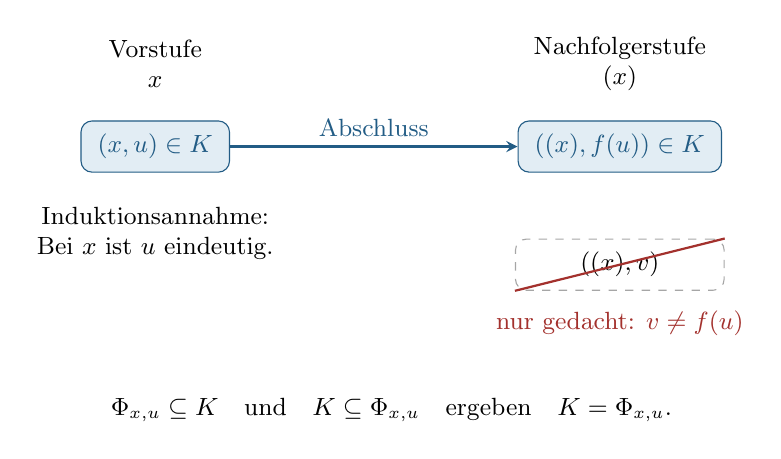
\begin{tikzpicture}[x=1cm,y=1cm,font=\small,>=stealth,
    pair/.style={draw=dedekindblue,fill=dedekindshade,
      rounded corners,minimum height=.65cm,inner xsep=6pt,
      text=dedekindblue}]
    \node[align=center] at (1.2,1.35)
      {Vorstufe\\\(x\)};
    \node[align=center] at (7.1,1.35)
      {Nachfolgerstufe\\\(\Succ(x)\)};

    \node[pair] (previous) at (1.2,.3) {\((x,u)\in K\)};
    \node[pair] (forced) at (7.1,.3) {\((\Succ(x),f(u))\in K\)};
    \draw[->,thick,dedekindblue]
      (previous)--node[above] {Abschluss}(forced);
    \node[align=center] at (1.2,-.8)
      {Induktionsannahme:\\Bei \(x\) ist \(u\) eindeutig.};

    % Kein behauptetes Element von K: nur der auszuschließende Kandidat.
    \node[draw=gray!70,dashed,rounded corners,
      minimum height=.65cm,minimum width=2.65cm,inner xsep=6pt]
      (extra) at (7.1,-1.2) {\((\Succ(x),v)\)};
    \draw[dedekindred,thick] (extra.south west)--(extra.north east);
    \node[align=center,text=dedekindred] at (7.1,-1.95)
      {nur gedacht: \(v\neq f(u)\)};

    \node[align=center] at (4.2,-3.05)
      {\(\Phi_{x,u}\subseteq K\)\quad und\quad
       \(K\subseteq\Phi_{x,u}\)\quad ergeben\quad
       \(K=\Phi_{x,u}\).};
  \end{tikzpicture}
  \par\smallskip\small\raggedright
  Der gestrichelte Eintrag bezeichnet nur ein mögliches zusätzliches Paar,
  dessen Zugehörigkeit zum Kern ausgeschlossen wird. Die Fixierungsmenge
  \(\Phi_{x,u}\) lässt bei \(\Succ(x)\) allein den Wert \(f(u)\) zu
  und erfüllt nach dem Beweis weiterhin die Admissibilitätsbedingungen.
  Aus ihrer Definition folgt \(\Phi_{x,u}\subseteq K\);
  ihre Admissibilität und die Minimalität von \(K\) liefern die umgekehrte
  Inklusion. Daher kann der Kern kein solches zusätzliches Paar enthalten.
  Das Bild setzt keine Eindeutigkeit in weiteren Stufen voraus.
  \end{minipage}\par\medskip
}
